\chapter{Attacking Machine Learning Systems}

In this chapter, we present approaches for attacking machine learning algorithms with adversarial techniques presented in the previous chapter. We discuss that the knowledge of the architecture and weight parameters is sufficient to derive adversarial samples against DNNs. Further discussion goes into black box attacks where the attack has minimal information about the underlying system. The discussion is then closed with how model's knowledge can be transferred between different algorithms/techniques.


\section{Transferability}

Papernot (2015) presented that many adversarial examples crafted to fool one specific model are also likely to affect another different model. As long as the models were trained to perform the same task, knowledge can be transferred when querying the victim model, namely oracle, to label a synthetic training set for the substitute.

The machine learning transferability property constitutes a threat vector for many state of the art methods, thus, one should be able to quantify most vulnerable classes of models by generating accurate comparison of the attack surface of each class. Attacks can, however, depend on some specific information of the target as shown in Table ~\ref{tbl:attack_info}. Techniques can mainly be split into both Intra-Technique and Cross-Technique. These are discussed in more details on the following sections.

\vskip 1cm

\begin {table}
\begin{tabular}{|c|c|}
	\hline 
	Model Parameters (Weights and Biases) & Have full access to model wieghts \\ 
	\hline 
	Model Architecture / Type & Know what the model looks like \\ 
	\hline 
	Training data & Understand the data domain \\ 
	\hline 
	Oracle/Black box & Query model with input X, get label Y \\ 
	\hline 
	
\end{tabular} 
\caption {How Much Information is needed to fool a model?}
\label{tbl:attack_info}
\end {table}

\medskip



\section{Intra-technique transferability}

The Intra-technique transferability is done by reproducing the learning process between two identical algorithms \cite{papernot2016transf}. Even though, the algorithms can differ in terms of architecture, they are still based on the same fundamental learning concept. For example, algorithms could be categorized into three different classes: differentiable algorithms like DNN and Logistic regressions, lazy learners like KNN and non-differentiable models like SVM and Decision Trees. Therefore, this technique consists of keeping the same learning method while differing the hyperparameters/architecture and using queried subset of the training data to train the local model. 



In order to make a comparison between these techniques, Papernot N. et. al (2015) \cite{papernot2016transf} created five different dataset models of the MNIST to train the algorithms and compare how they perform when using different and same models of training data. All models had non-negligible vulnerability to this kind of approach. While DNN and LR were highly vulnerable to these attacks, SVM, DT and KNN were more robust achieving better overall resillience. The results have led to the hypothesis that non-differentiable techniques are more robust to black-box attacks using locally generated adversarial sample in between two algorithms of the same type \cite{papernot2016}. Figure ~\ref{fig:intra} shows classification performance when using intra-technique methods.

\begin{figure}[!h]
\centering
	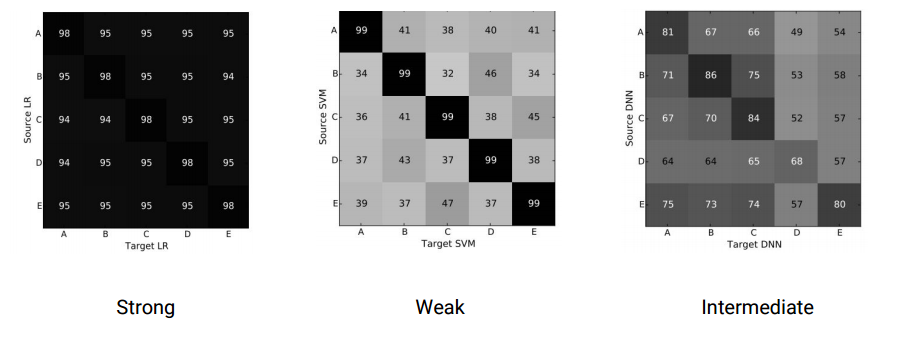
\includegraphics[scale=0.6]{intra.png}
\caption{Knowledge transfer level using Intra-Technique Transferability \cite{papernot2016transf}}
\label{fig:intra}
\end{figure}


\section{Cross-technique transferability}
Cross-Technique transferability was referred as the knowledge transfer between two different machine learning techniques. This problem has a higher degree of difficulty than the method shown on section \ref{subsubsec:intra} as it involves models using possibly very different techniques like DNNs and Decision trees. Yet, this can be seen as quite strong phenomenon to which techniques like Logistic Regression, Support Vector Machines and Decision Trees along with Ensemble based models are extremely vulnerable \cite{papernot2016transf}.

Papernot N. et. al \cite{papernot2016transf} have shown a strong but heterogeneous phenomenon. While DNN's ended up as being the most robust of the methods with misclassification rates varying between 0.82\% and 38.27\%, Decision Trees were the most vulnerable with rates from 47.20\% to 89.29\%. Interesting enough, ensemble methods -- focused on measuring the output of all the "experts" in the group -- have shown quite vulnerable to the experiment. The hypothesis is that the technique explores the individual vulnerability within each of the ensemble methods.

\begin{figure}[!h]
\centering
	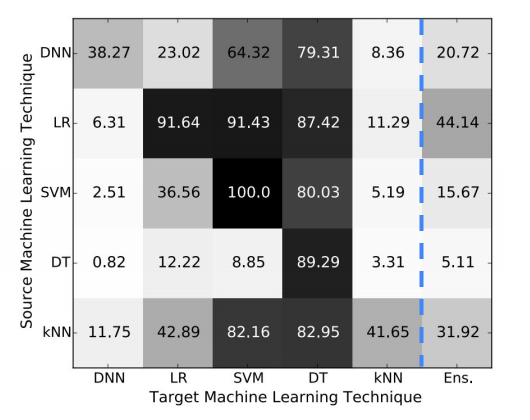
\includegraphics[scale=0.6]{cross.png}
\caption{Knowledge transfer using Cross-Technique Transferability and Ensemble Methods \cite{papernot2016transf}}
\label{fig:cross}
\end{figure}
\section{Black-box Attacks}
Black-Box attack to machine learning systems alleviates the dependence on knowing both victims training data and model information. This method solely depends on accessing the label assigned by the target for any chosen input. The strategy consists of learning a substitute for the target model using a synthetic dataset generated by the adversary and labeled by the observed victim, namely here, the Oracle \cite{papernot2016}.

Training the substitute model that approximates the Oracle poses some challenges. Selecting an architecture for the substitute ends up in being an arbitrary process, as one should try different models and evaluate the one with the best result. Generating the synthetic dataset needs to limit the number of queries sent to the oracle so the approach is tractable. 

Experiments from Papernot et al. (2016) were performed against real-world remote systems in order to validate the effectiveness of such attacks. The results have shown that systems using DNNs are usually more robust and require more queries to have the substitute being able to generate samples that are misclassified by the oracle.

\begin{table}[!h]
\centering
	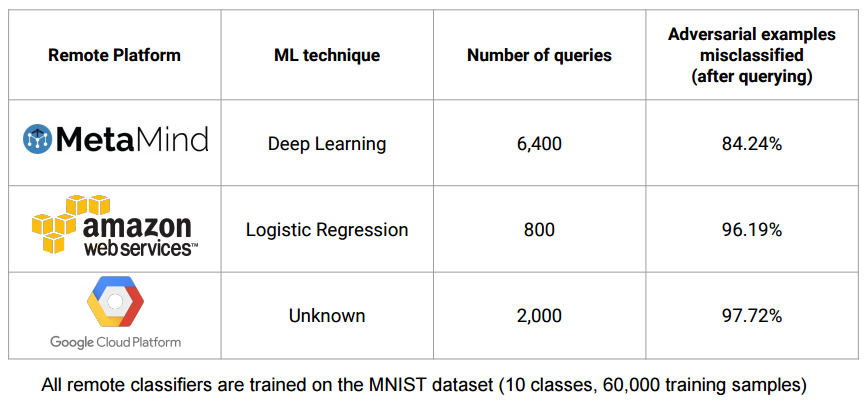
\includegraphics[scale=0.7]{black_box.png}
\caption{Black-Box attacks results against real world systems}
\label{tbl:black_box}
\end{table}

\section{Unrecognizable Images}\label{subsec:unrec}

Adversaries, on the other hand, are not only comprised of small perturbations on known images. Nguyen et al (2015) presented a method for producing images that are unrecognizable to humans, but are nonetheless labeled as recognizable objects by DNNs \cite{nguyen2015}. For instance, a DNN would classify a noise-filled image crafted using their technique with high confidence. These images were named $fooling images$ since they do not have a source class but are crafted solely to perform a targeted misclassification attack.

\begin{figure}[!h]
	\centering
	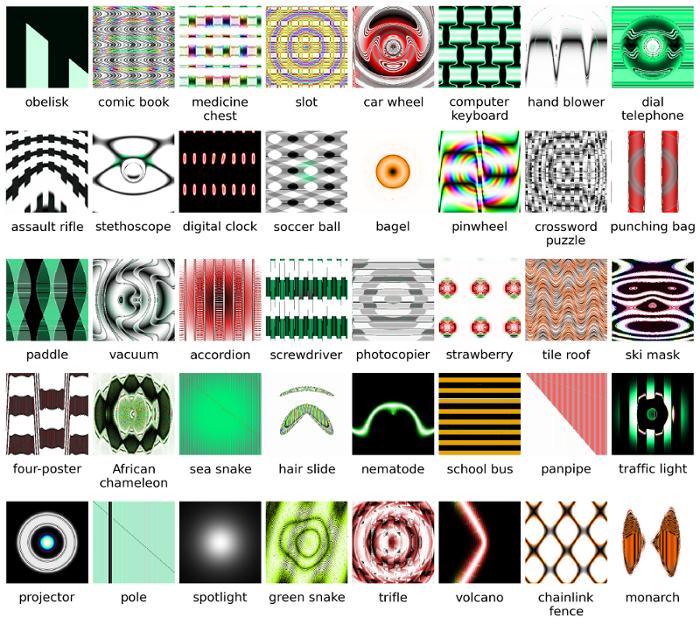
\includegraphics[scale=1.]{unrec_images.png}
	\caption{Examples of noisy images classified with high confidence \cite{nguyen2015}.}
	\label{fig:unrec_images}
\end{figure}


\section{Adversarials in the Physical World}\label{sec:physical}

All the aforementioned techniques were based into feeding information directly into machine learning systems. Such model only takes into consideration situations in which attacks take place entirely within the computer. For instance, these techniques could be used by attackers to avoid spam filters or malware detectors. Even though the study is utterly relevant, a recent study conducted by \cite{goodfellow2016} have shown that it is possible to craft adversarial samples in order to perform attacks on machine learning systems which are operating in the physical world.

Although the Fast Gradient Sign method have been successful on crafting adversarial examples, there are some extensions of the method that can be used in order to create perturbations that are more likely to work in the physical world. Firstly, \cite{goodfellow2016} introduced a variation named \textit{Basic Iterative Method}. This technique consists of applying the fast method multiple times with small step sizes and making sure that all pixels are within a $\epsilon$-neighbourhood of the original image. The number of iterations was chosen heuristically with goals of being sufficient enough to have the adversarial example reaching the edge of the $\epsilon$ max-norm.

In order to perform experiments, clean photos of adversarial examples created using the three methods were taken and fed into a machine learning system using Deep Convolutional Neural Networks (Inception V3). Adversarial Images created using the "fast" method were more robust when compared to the iterative methods. The hypothesis behind the result is that iterative methods create more subtle perturbations that can be easily be destroyed by the photo transformation process (Photo Printing as described above). Overall, it could be expected that about 2/3 of the images would be top-1 misclassified and about 1/3 top-5 misclassified by the fast method using an $\epsilon$ of 16.

Adversarial examples is not only feasible on digital attacks but also on physical world scenarios. By using the correct perturbation algorithm with optimized hyperparameters one can use printed digital photos to fool day-to-day machine learning systems. As more and more machine learning is becoming part of our environment, techniques for avoiding such attacks need to be developed so these systems can become less vulnerable to any kind of attack.

\section{Defending Against Adversarial Attacks}\label{sec:robustness}

Since adversarials are exploiting intrinsic network properties, these could also be used when training a network in order to develop robustness to possible examples crafted using the same methods. By using the worst case perturbation of a point \textit{x} instead of \textit{x} itself it is possible to derive an equation that includes the perturbation within its objective function. This form of training was able to reduce the error rate of adversarial examples from 0.94\% to 0.84\% \cite{goodfellow2014}. Adversarial training can be seen as a way of teaching the model how an adversarial looks like and that it should be able to generalize not only normal images but also perturbed ones. Another way of creating robustness was developed by using bayesian non-parametric methods. Estimating the confidence that an input is natural during the training phase can lead the network to generate priors that take into account adversarial perturbation of points \cite{billovits}. 

$$ C(\omega,x,y) = \alpha C(\omega ,x,y) + (1-\alpha )C(\omega ,x+\epsilon sign(\nabla_{x}C(\omega,x,y))$$

Most adversarial construction techniques use the gradient of the model to make an attack. In other words, they look at a picture of an airplane, they test which direction in picture space makes the probability of the "cat" class increase, and then they give a little push in that direction. These are hard to defend against because it is hard to construct a theoretical model of the crafting process. These examples are solutions to an optimization problem that is non-linear and non-convex for many ML models, including neural networks. Since there is no good theoretical tools for explaining the solutions of these complicated problems, it makes it very hard to make any kind of theoretical argument that a defense can improve an algorithm from a set of adversarial examples.